\clearpage

\setcounter{chapter}{2}
\setcounter{section}{0}

% Add the chapter to table of contents
\addcontentsline{toc}{chapter}{\numberline{2}Rethinking Democratization: Beyond Access to Preservation}

\pagestyle{fancy}
\fancyhf{} % Clear all header and footer fields
\fancyhead[L]{\footnotesize\textit{Ars Post Faber: Digital Fabrication Democratization Through Embodied Knowledge Preservation}}
\fancyfoot[C]{\thepage} % Page number in footer center
\renewcommand{\headrulewidth}{0pt}
\renewcommand{\footrulewidth}{0pt}

\noindent
{\Large\textbf{Chapter 2: Rethinking Democratization: Beyond Access to Preservation}}
\vspace{0.3cm}
\hrule
\vspace{0.8cm}
\label{ch:democratization}

% Set no paragraph indentation
\setlength{\parindent}{0pt}

The historical trajectory examined in Chapter 1 has showed how creative agency has been systematically redistributed from unified practice to contemporary digital workflows. This analysis raises the question: if digital fabrication technologies possess unprecedented capabilities for material manipulation and geometric exploration, why do they continue to perpetuate the same distributed agency frameworks that eliminated adaptive authority? The answer lies in how the "democratization" itself has been conceptualized within digital fabrication discourse.

\vspace{0.5cm}

Rather than addressing the organizational structures that fragment creative agency, contemporary digital fabrication has pursued democratization primarily through expanded access to scaled-down industrial tools. This chapter will examine how this access-centered approach, while achieving remarkable quantitative success, fails to address the deeper structural issues identified in the historical analysis. By tracing the evolution from access-based democratization toward preservation-centered approaches, this chapter will try to pursue a reconceptualization of what democratic making might mean in digital contexts.

\section{The Access Paradigm and Its Achievements}

This access-centered understanding of democratization has become the dominant paradigm within contemporary digital fabrication discourse. Neil Gershenfeld's\footnote{Neil Gershenfeld is a physicist at MIT who's the director of the Center for Bits and Atoms (CBA) and pioneered the global FabLab movement. His work focuses on the intersection of physical and digital systems, advocating for "personal fabrication" as a means to democratize access to manufacturing capabilities.} vision for FabLabs\footnote{FabLabs (Fabrication Laboratories) are digital fabrication workshops that provide public access to tools for invention, prototyping and local production. Originally conceived at MIT's Center for Bits and Atoms, FabLabs follow a global charter emphasizing open access, education, and local innovation while connecting to a worldwide network of collaborative spaces.} promised "personal fabrication" enabling "almost anyone to make almost anything" \citep{gershenfeld2007}, positioning digital fabrication as the natural evolution of personal computing—bringing the same accessibility that desktop computers brought to information processing into the realm of physical manufacturing. This vision emphasized scaling down industrial production capabilities to individual users, making sophisticated fabrication tools available in community workshops and educational institutions.

\begin{figure}[H]
\centering

\includegraphics[width=0.4\textwidth]{figures/chapter2/fablab.png}
\caption{Fab Labs Logo. Source: \cite{fabfoundation2024}}
\label{fig:fablab_tools}
\end{figure}

Building on this foundation, the broader maker movement, as articulated by Mark Hatch, advocated for "radically democratizing access to the tools of innovation" \citep{hatch2013}, framing making as both a form of personal empowerment and economic opportunity. Hatch's manifesto positioned the maker movement as a response to mass production's alienation, promising that widespread access to fabrication tools would restore individual agency in production while fostering innovation and entrepreneurship at the grassroots level.

\begin{figure}[H]
\centering
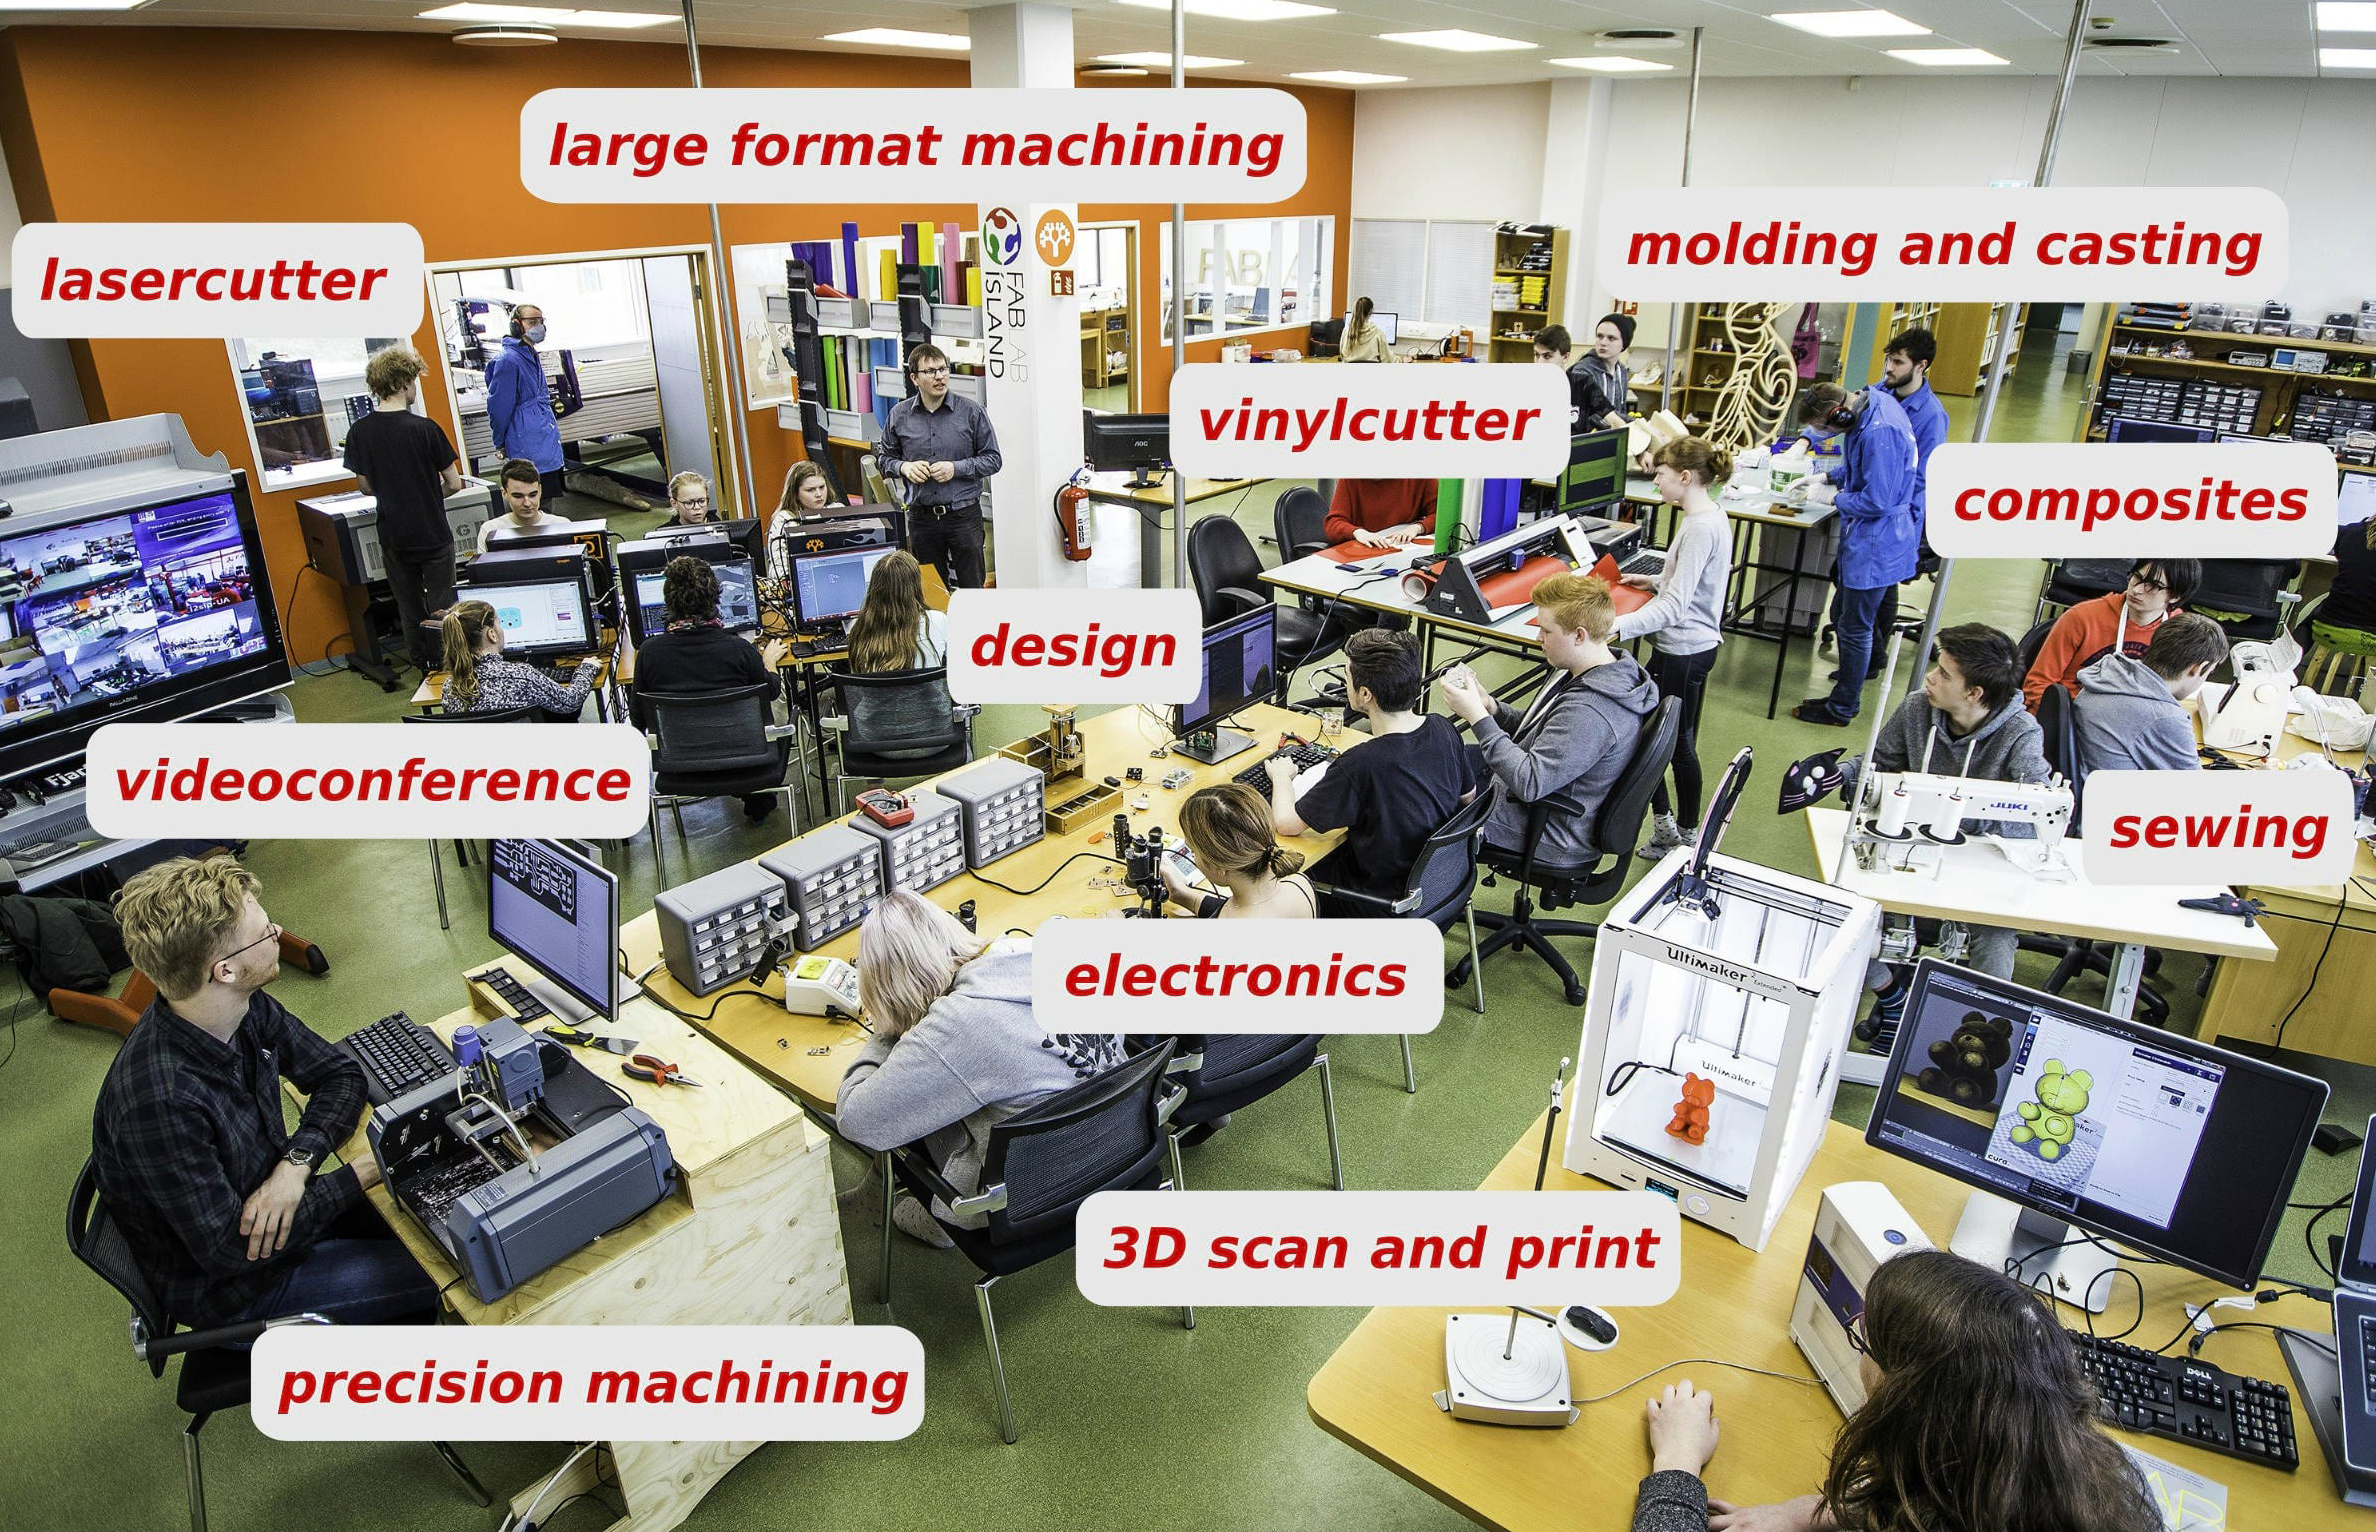
\includegraphics[width=1\textwidth]{figures/chapter2/fablab_tools.jpg}
\caption{Tools in a Fab Lab. Source: \cite{fabfoundation2024}}
\label{fig:fablab_tools}
\end{figure}

This approach has achieved remarkable quantitative success: from fewer than 50 FabLabs worldwide in 2009 to over 2,000 by 2023 \citep{fabfoundation2024}, there's been an unprecedented expansion of access to sophisticated production capabilities.

\begin{figure}[H]
\centering
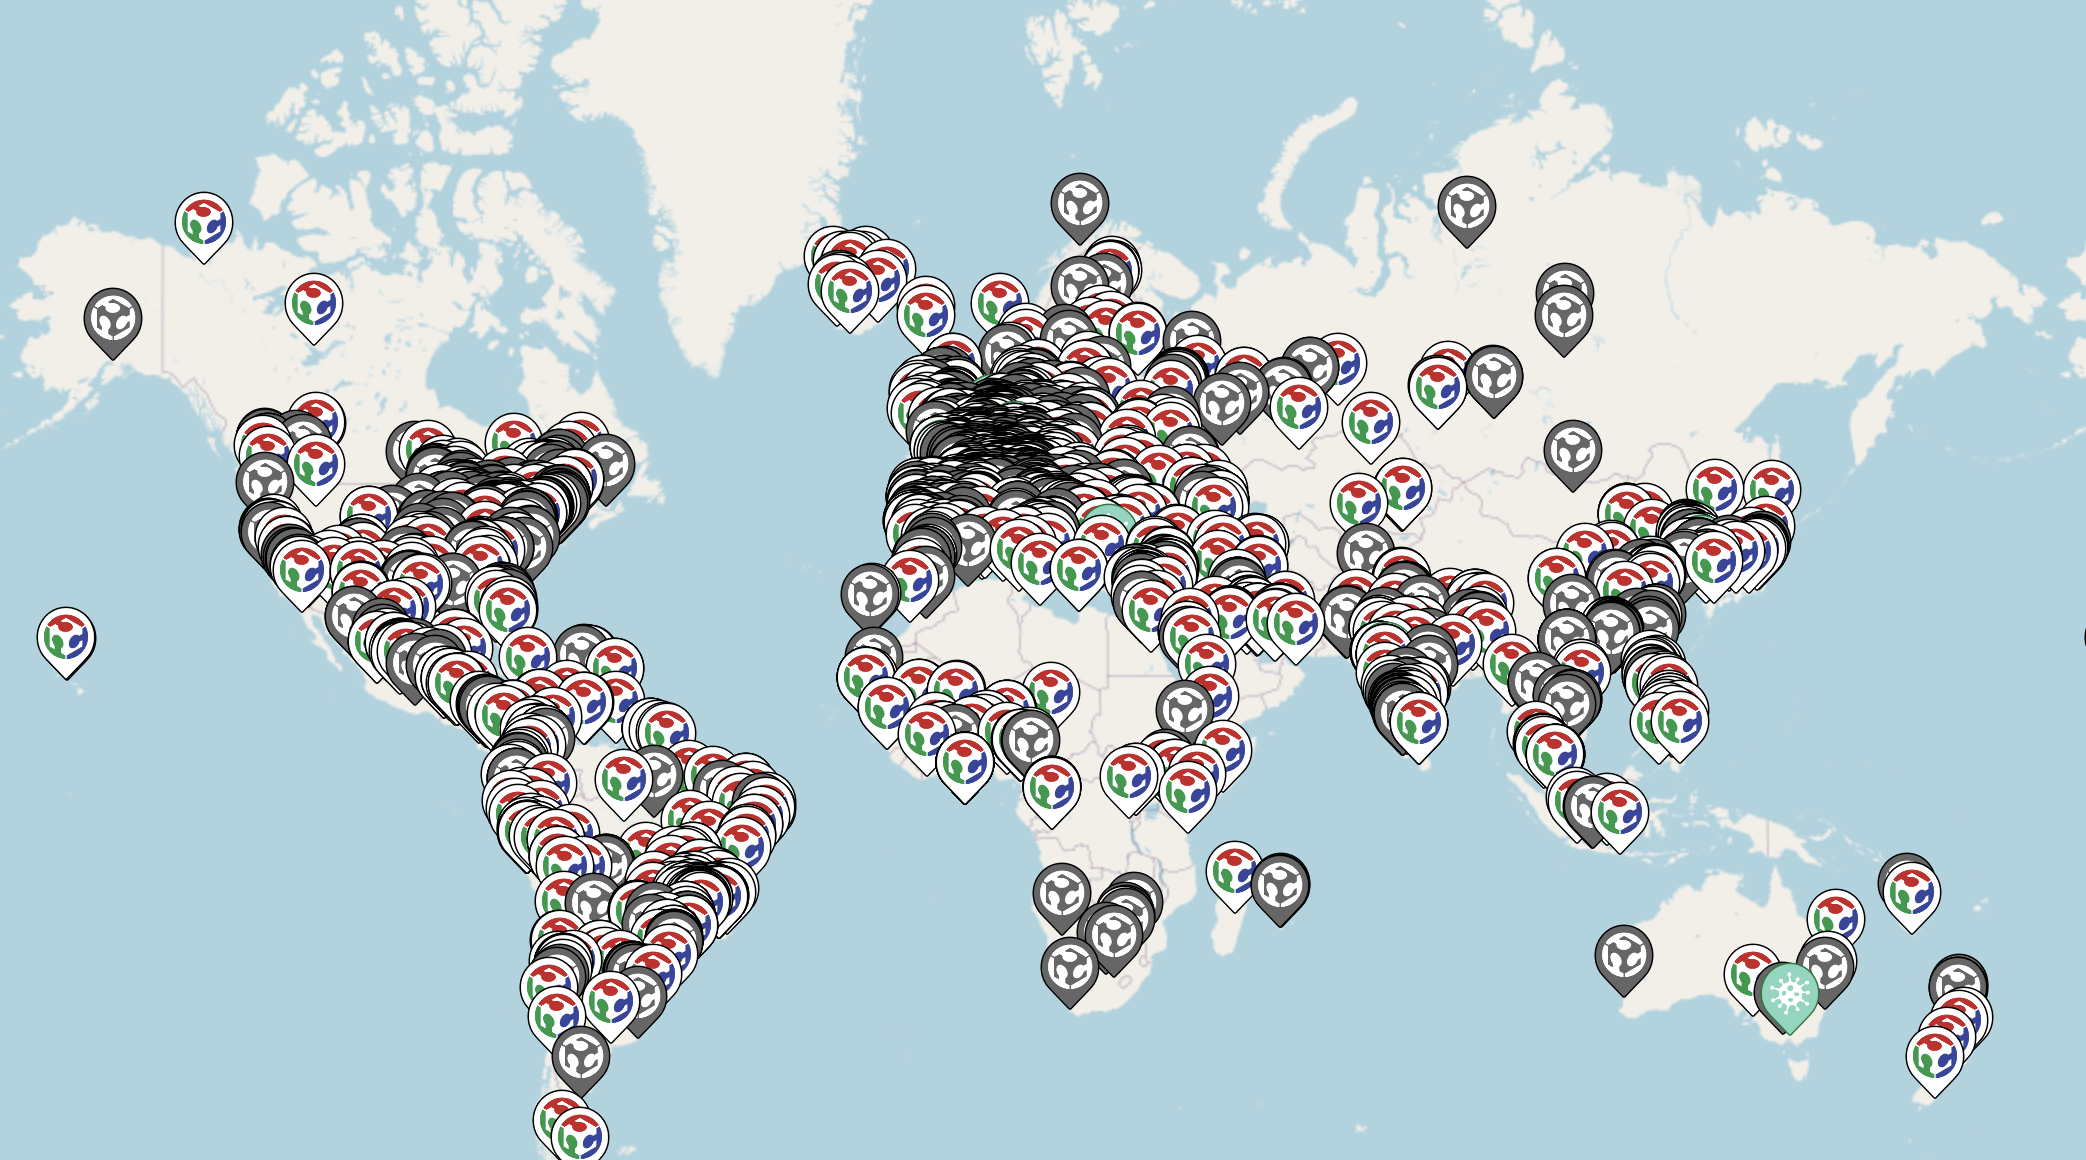
\includegraphics[width=1\textwidth]{figures/chapter2/fablabsmap.png}
\caption{Global distribution of FabLabs. Map showing the locations of FabLabs around the world. Source: \cite{fabfoundation2024}}
\label{fig:fablabs_map}
\end{figure}

This democratization of digital fabrication extends beyond physical tools to software infrastructures. Open-source\footnote{Open-source software is developed with publicly accessible source code, allowing users to modify, improve the software and in some cases even distribute it.} and free CAD alternatives like FreeCAD\footnote{FreeCAD is a parametric 3D CAD modeler designed for mechanical engineering and product design, available as free and open-source software.}, Blender\footnote{Blender is an Open-Source 3D creation suite supporting modeling, animation, rendering, and video editing, mainly used for animation but increasingly used for CAD applications.} or TinkerCAD\footnote{TinkerCAD is a web-based 3D design application developed by Autodesk, designed for beginners with simplified modeling tools and browser-based accessibility.} combined with educational programs to know how to use the tools, have reduced barriers to digital design literacy. Contemporary maker spaces enable individual access to CNC machines\footnote{Computer Numerical Control (CNC) machines use computer-controlled cutting tools to precisely shape materials like wood, metal, and plastic from digital designs.}, 3D printers\footnote{3D printers create physical objects by depositing material layer by layer based on digital 3D models, enabling rapid prototyping and small-scale production.}, and laser cutters\footnote{Laser cutters use focused laser beams to cut or engrave materials with high precision, commonly used for creating flat parts from sheet materials like wood, acrylic, and metal.} for modest fees (sometimes even for free), genuinely transforming the economic conditions of making.

\begin{figure}[H]
\centering

\includegraphics[height=4.4cm]{figures/chapter2/Blender.png}
\hspace{1.5cm}

\includegraphics[height=4.8cm]{figures/chapter2/freeCAD.png}
\caption{Open-source CAD alternatives: Blender and FreeCAD logos. Sources: \citet{blender2024}, \citet{freecad2024}}
\label{fig:opensource_cad_logos}
\end{figure}

Yet this access-focused paradigm highlights certain limitations when examined against historical precedents of successful democratization movements. The expansion of who can use fabrication tools does not address how those tools structure agency within making processes. As Tanenbaum et al. observe, maker practices still depend heavily on existing industrial infrastructure and face challenges "when it comes to scaling up production and distribution" \citep{tanenbaum2013}.

\section{The Preservation Problem: What Access Cannot Address}

While the quantitative expansion of fabrication access represents genuine progress, it reveals limitations in how democratization has been conceptualized. What contemporary digital fabrication lacks is what this research identifies as a preservation problem: the loss of tacit knowledge and embodied practices that characterize skilled making. This goes beyond the historical fragmentation patterns analyzed in Chapter 1 to encompass how knowledge itself is transmitted, maintained, and evolved within making communities.

\vspace{0.5cm}

Richard Sennett's analysis of craftsmanship emphasizes that "the desire to do something well for its own sake" \citep{sennet2009} requires forms of embodied learning that resist systematic codification. Unlike explicit knowledge that can be documented in manuals or encoded in software, tacit knowledge emerges through sustained engagement with materials, tools, and techniques.

\vspace{0.5cm}

Contemporary digital fabrication workflows eliminate opportunities for this knowledge transmission. While FabLabs and maker spaces provide access to sophisticated tools, they typically operate through standardized tutorials and predetermined project sequences that prioritize rapid skill acquisition over deep material understanding. The emphasis on "democratizing" access often translates into simplifying workflows to reduce learning curves, eliminating the complex, time-intensive processes through which tacit knowledge traditionally develops.

\begin{figure}[H]
\centering
\includegraphics[width=1\textwidth]{figures/chapter2/3d_Printer.png}
\caption{3D Printer at Fab Lab Bcn. Source: Author}
\label{fig:fablabs_map}
\end{figure}

This preservation problem manifests through persistent organizational structures that extend beyond individual tool use. Despite the collaborative and educational dimensions of maker spaces, the workflow architecture maintains the distributed agency pattern traced in Chapter 1. Creative decisions remain concentrated in separate design phases, while material execution follows predetermined procedures that eliminate opportunities for the responsive adaptation. The result is a democratization that provides access to tools without preserving the knowledge systems that enable those tools to support genuine creative agency.

\vspace{0.5cm}

The insight that emerges from this analysis is that democratization cannot be achieved through access alone, it requires organizational innovation that preserves the continuity of creative decision-making throughout the making process. This shifts focus from who can use fabrication tools to how those tools can be structured to maintain what was identified in Chapter 1 as unified agency. 

\section{Redefining Democratization: Process Over Access}

Through the analysis of the preservation problem it's possible to raise the question about how "democratization" has been conceptualized within digital fabrication discourse. While the term implies expanding democratic participation, current approaches, as mentioned, focus primarily on access expansion rather than examining what democratic participation actually requires. Before proposing alternative models for fabrication democratization, it becomes necessary to question what "democracy" itself demands and how those requirements might apply to making contexts.

\begin{figure}[H]
\centering
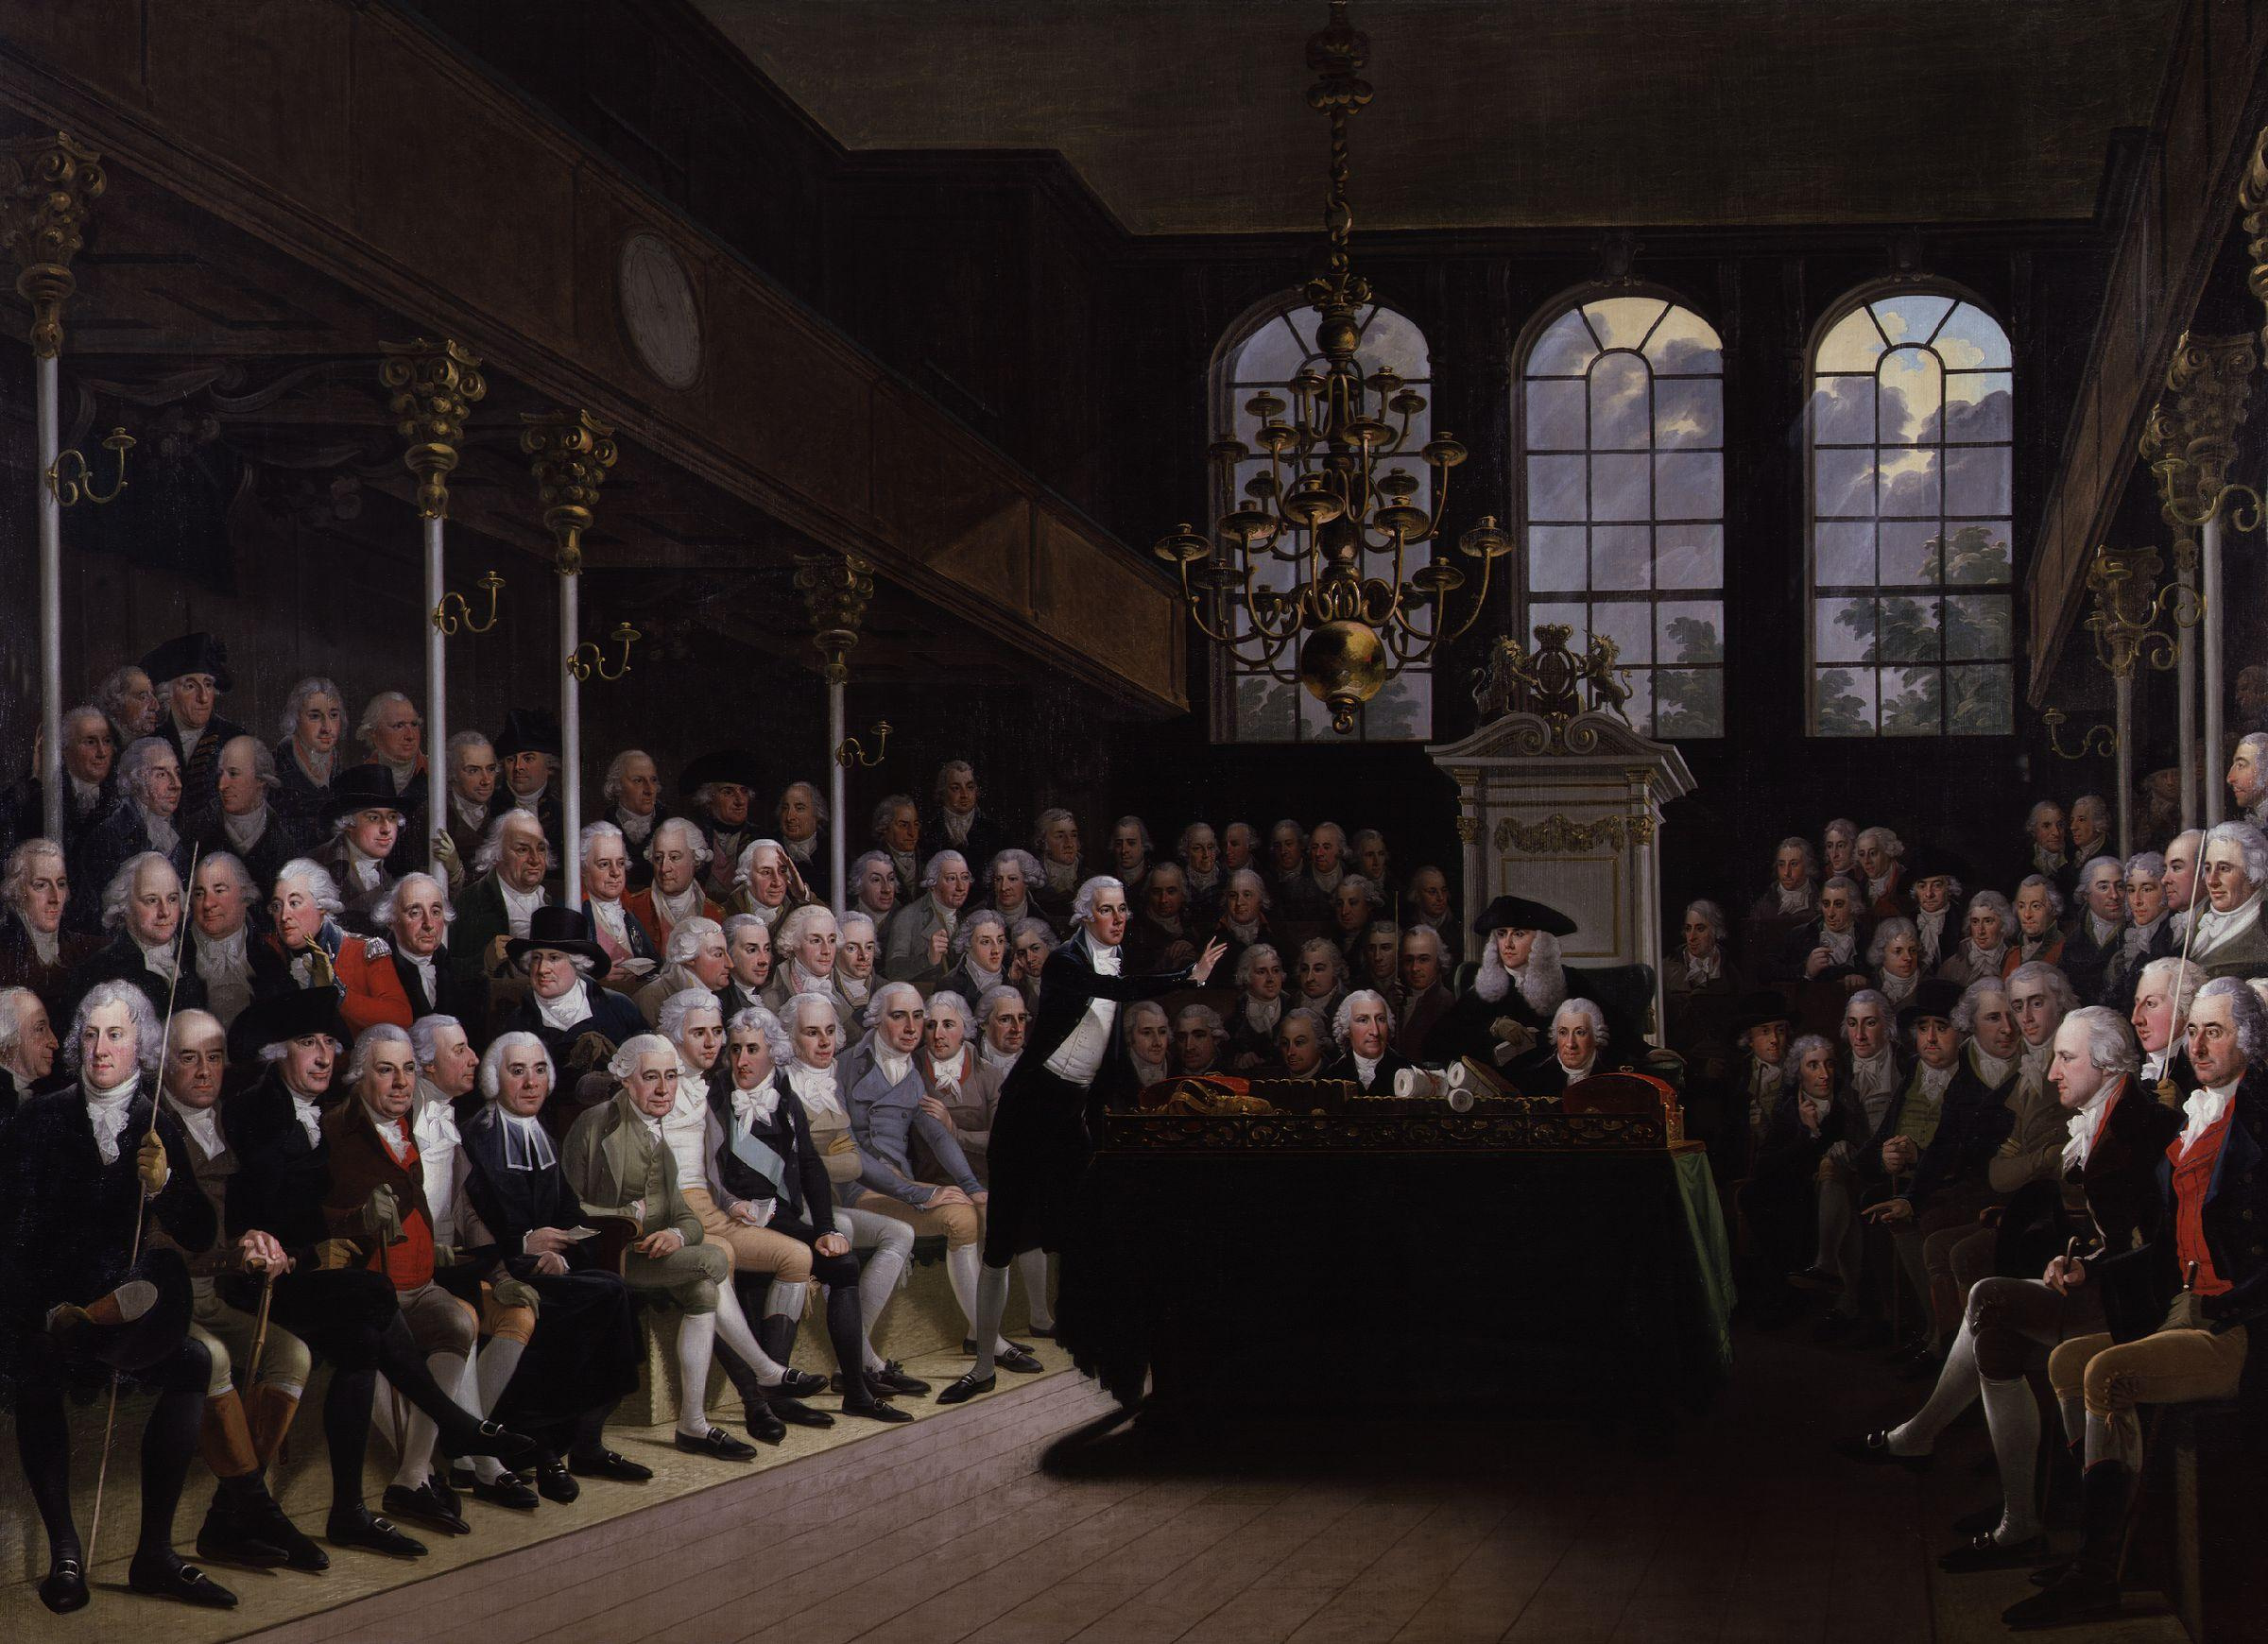
\includegraphics[width=1\textwidth]{figures/chapter2/The_House_of_Commons_1793-94.jpg}
\caption{William Pitt the Younger addressing the Commons in \textit{The House of Commons, 1793–94}. Source: \citet{hickel_commons_1794}}
\label{fig:house_of_commons_1794}
\end{figure}

The analysis of different precedents and patterns suggest that democratization movements across multiple domains initially focus on access expansion before recognizing deeper structural challenges. Political democratization, educational reform, and cultural preservation movements all showcase patterns that would align with it: early phases emphasize expanding participation within existing systems, while later phases require fundamental transformation of the systems themselves. For instance, political democratization initially focused on expanding voting rights, but later required systematic changes like proportional representation systems such as the D'Hondt method\footnote{The D'Hondt method is a proportional representation electoral system that allocates seats based on vote share, developed to ensure more democratic representation beyond simple majority voting.} to ensure genuine democratic representation rather than mere voting access. Similarly, educational democratization moved beyond simply expanding school enrollment to developing pedagogical approaches that understand and accommodate diversity in the classroom, adapting curricula to different learning styles and cultural backgrounds rather than imposing standardized approaches. These precedents suggest that fabrication democratization may be encountering similar limitations inherent to access-based approaches.

\vspace{0.5cm}

Rather than assuming that broader tool access automatically produces democratic participation, the following analysis will examine what democracy actually requires and how those requirements might inform alternative approaches to fabrication democratization. By analyzing democratic theory alongside cross-cultural preservation practices, this chapter will attempt to develop frameworks for distinguishing between superficial access and substantive democratic participation in production processes.

\subsection{Deconstructing "Democratization": What Democracy Actually Requires}

The theoretical framework established requires a deeper examination of the term "democratization" itself and its specific application to fabrication contexts. While democratic theory provides extensive analysis of political participation, its principles have been applied to fabrication with insufficient critical examination of what democratic participation might actually require within making processes. The word "democracy" derives from the Greek {\greekfont δημοκρατία} (demokratia) demos (people) + kratos (power/rule), meaning rule by the people. This etymology suggests that democratization involves the distribution of ruling authority rather than expanded access to predetermined systems, a distinction with big implications for how fabrication democratization should be conceptualized.

\begin{figure}[H]
\centering
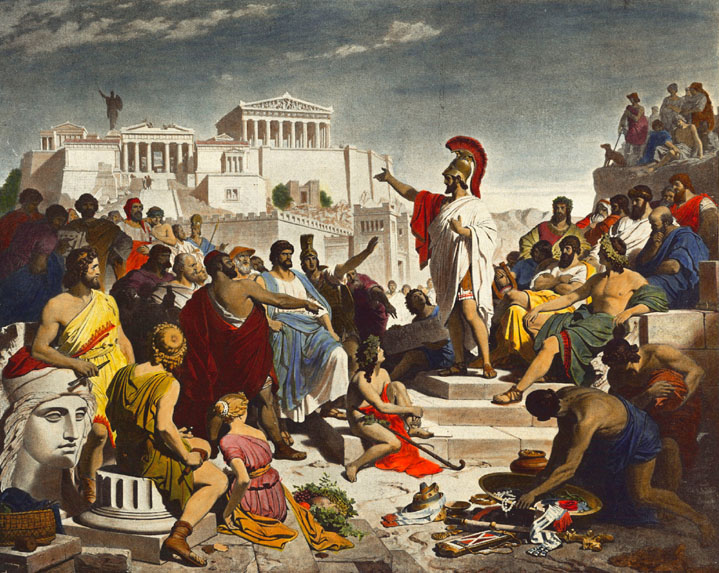
\includegraphics[width=0.8\textwidth]{figures/chapter2/Discurso_funebre_pericles.png}
\caption{Nineteenth-century painting by Philipp Foltz depicting the Athenian politician Pericles delivering his famous funeral oration in front of the Assembly. Source: \citet{foltz_pericles}}
\label{fig:pericles_funeral_oration}
\end{figure}

Political democracy, at its core, requires the distribution of decision-making authority among participants rather than merely access to predetermined decision-making processes. As Robert Dahl's\footnote{Robert A. Dahl (1915--2014) was an American political theorist whose work on democratic theory, shaped contemporary understanding of democratic systems and citizen engagement.} foundational analysis demonstrates, democratic systems must provide "effective participation" \citep{coglianese1990} where citizens have "basic political rights and liberties, such as free expression, and allows persons to live under laws of their own choosing" \citep{coglianese1990}, and enlightened understanding enabling informed choice among alternatives. Crucially, democracy requires what Dahl terms "final control over the agenda" \citep{mayhew2017}, the authority to determine not just outcomes within predetermined options, but the capacity to define what questions get asked and how they are framed. Distinguishing genuine democratic participation from consultative processes that solicit input within predetermined parameters while concentrating agenda-setting authority elsewhere.

\vspace{0.5cm}

Applied to fabrication contexts, this analysis reveals that current maker spaces, despite their collaborative ethos, preserve a fabrication autocracy, a system that concentrates creative authority in separate design phases while relegating material execution to predetermined procedures that eliminate participant agency. Genuine fabrication democratization would require the distribution of creative decision-making authority throughout making processes, enabling makers to exercise "final control over the agenda" not just in initial design specification, but in determining how fabrication workflows themselves operate and evolve in response to material conditions and emergent discoveries.

\subsection{The Representation Problem in Fabrication Democracy}

Having established that genuine democratization requires the distribution of decision-making authority rather than mere access expansion, it becomes necessary to examine how such authority might be structured within fabrication contexts. Political democracy usually confronts the challenge of representation: how to enable large-scale collective decision-making while preserving individual agency? This requires sophisticated institutional frameworks, electoral systems, deliberative processes, and constitutional protections that mediate between individual preferences and collective outcomes without eliminating personal autonomy.

\vspace{0.5cm}

Fabrication democratization faces analogous representational challenges: how to enable collective access to sophisticated manufacturing capabilities while preserving individual makers' authority to determine their own creative processes? Yet current digital fabrication has developed no equivalent to democratic political institutions. Instead, it has adopted  a technocratic representation, expert-designed software interfaces and standardized file formats that mediate between human intention and material execution while eliminating opportunities for maker input beyond initial design specification.

\vspace{0.5cm}

This technocratic approach mirrors Joseph Schumpeter's\footnote{Joseph Schumpeter (1883-1950) was an Austrian economist and politic who developed influential theories about capitalism and democratic systems.} theory of democracy as "competitive leadership" \citep{schumpeter1950}, a system that preserves formal democratic procedures while concentrating substantive decision-making authority within expert institutions. Just as this limited democracy enables citizen participation within predetermined choices while eliminating popular control over the agenda setting, just as current fabrication democratization enables maker participation within predetermined expert designed workflow structures while eliminating authority over how those structures have to be operated.

\subsection{Participatory Democracy and Making}

The technocratic representation reflects what participatory democratic theorists have long criticized in conventional political systems. Rather than accepting the limited model of democracy as competitive leadership, theorists like Carole Pateman advocate for democracy as active participation across all spheres of social life, "a society where all political systems have been democratised and socialisation through participation can take place in all areas" \citep{pateman1976}. Pateman argues that democratic capacity cannot be developed through formal instruction alone but emerges through the practice of exercising democratic authority in concrete contexts.

\vspace{0.5cm}

For fabrication democratization, out of this participatory approach can be extracted that creative agency develops itself through sustained engagement with decision-making throughout the making process rather than through standardized training in predetermined procedures. This would challenge the separation between tool designers and tool users that characterizes current maker spaces, and processes, requiring structures that enable makers to collectively determine how fabrication workflows themselves operate and evolve. Instead of accepting expert-designed workflow structures as fixed constraints, participatory fabrication would enable makers to exercise that "final control over the agenda".

\section{Deconstructing "Preservation": Beyond Cultural Heritage Models}

Out of the democracy framework outlined in this research can be assumed that genuine fabrication democratization requires preserving makers' capacity for ongoing creative authority rather than simply expanding access to predetermined tools. This shifts the focus from "democratization" as access provision to "democratization" as preservation of agency. But what kind of preservation enables rather than constrains democratic participation? The concept of "preservation" itself requires an examination, as its application to craft knowledge has been heavily influenced by cultural heritage frameworks that reproduce the same static approaches that align with access-based democratization.

\vspace{0.5cm}

Understanding preservation through cross-cultural perspectives can reveal assumptions embedded within Western conservation models and might highlight alternative approaches more suitable for maintaining the creative agency that democratic fabrication requires.

\subsection{Preservation as Dynamic Process vs. Static Conservation}

Traditional cultural preservation models, developed primarily for archaeological, crafts, and architectural contexts, emphasize conservation of existing artifacts and documentation of historical practices. This approach, rooted in western "museum culture", treats cultural objects as fixed entities requiring protection from change rather than as elements within ongoing living traditions that respond to new conditions and challenges.

\begin{figure}[H]
\centering
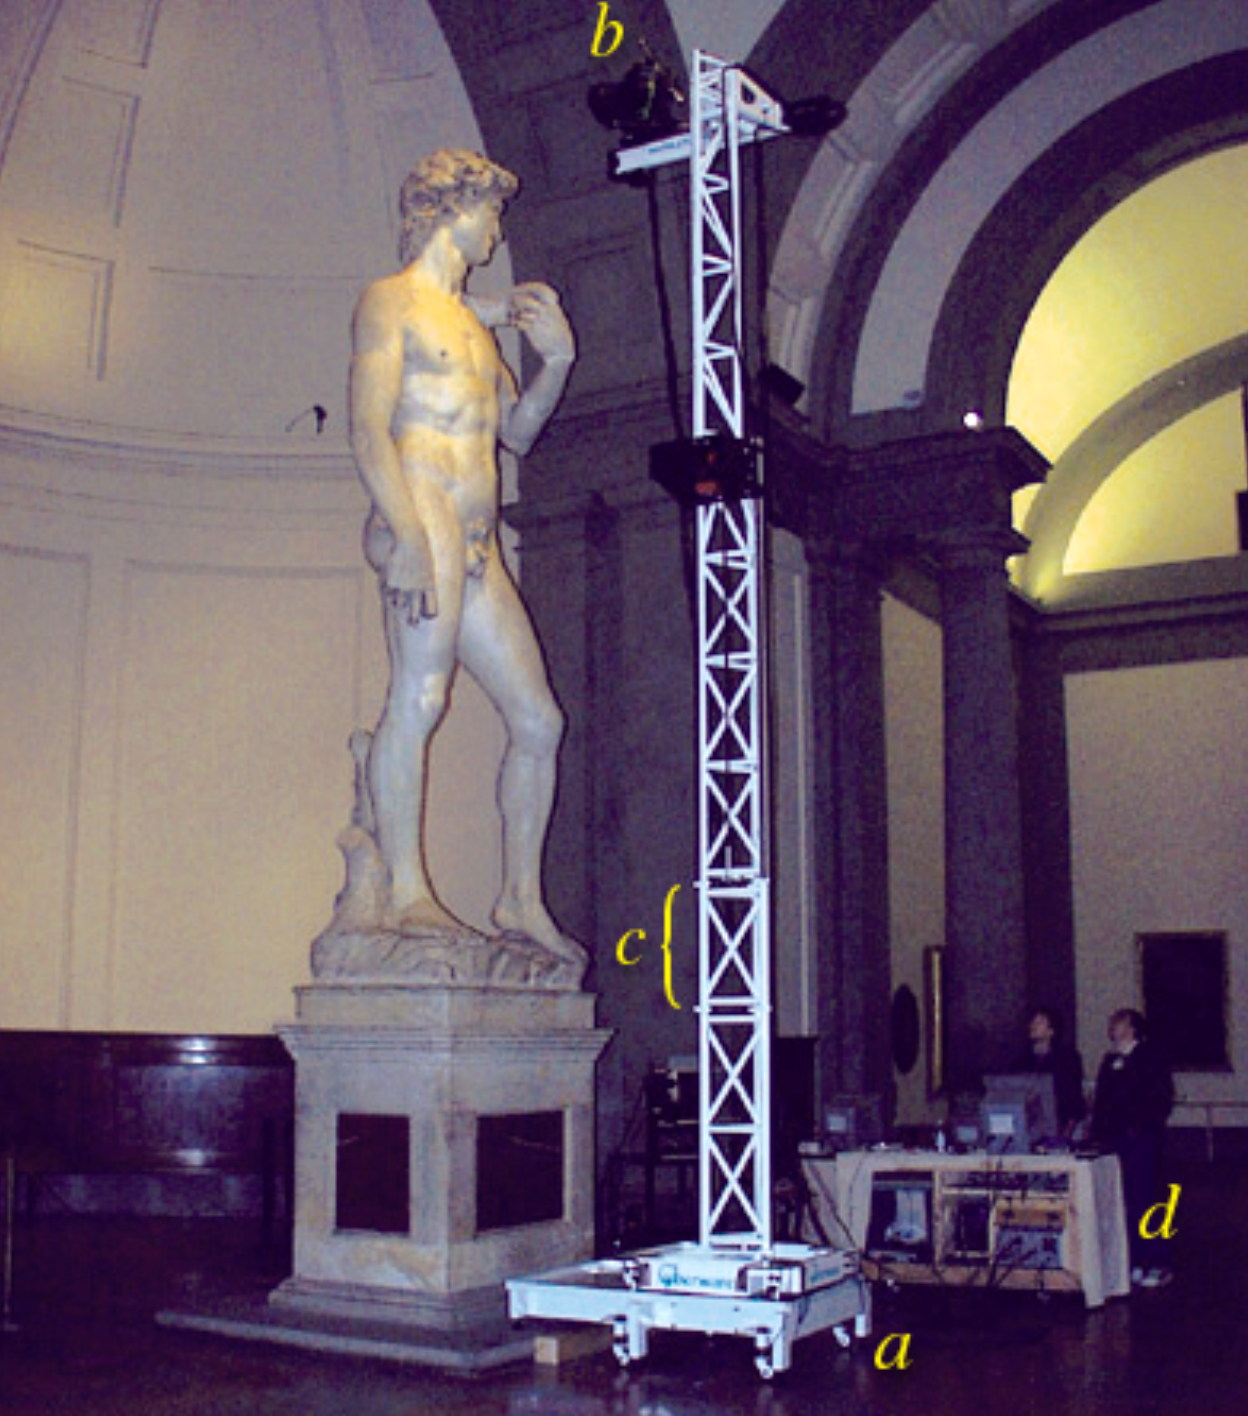
\includegraphics[height=9cm]{figures/chapter2/michelangelo_figure6.png}
\hspace{0.01cm}
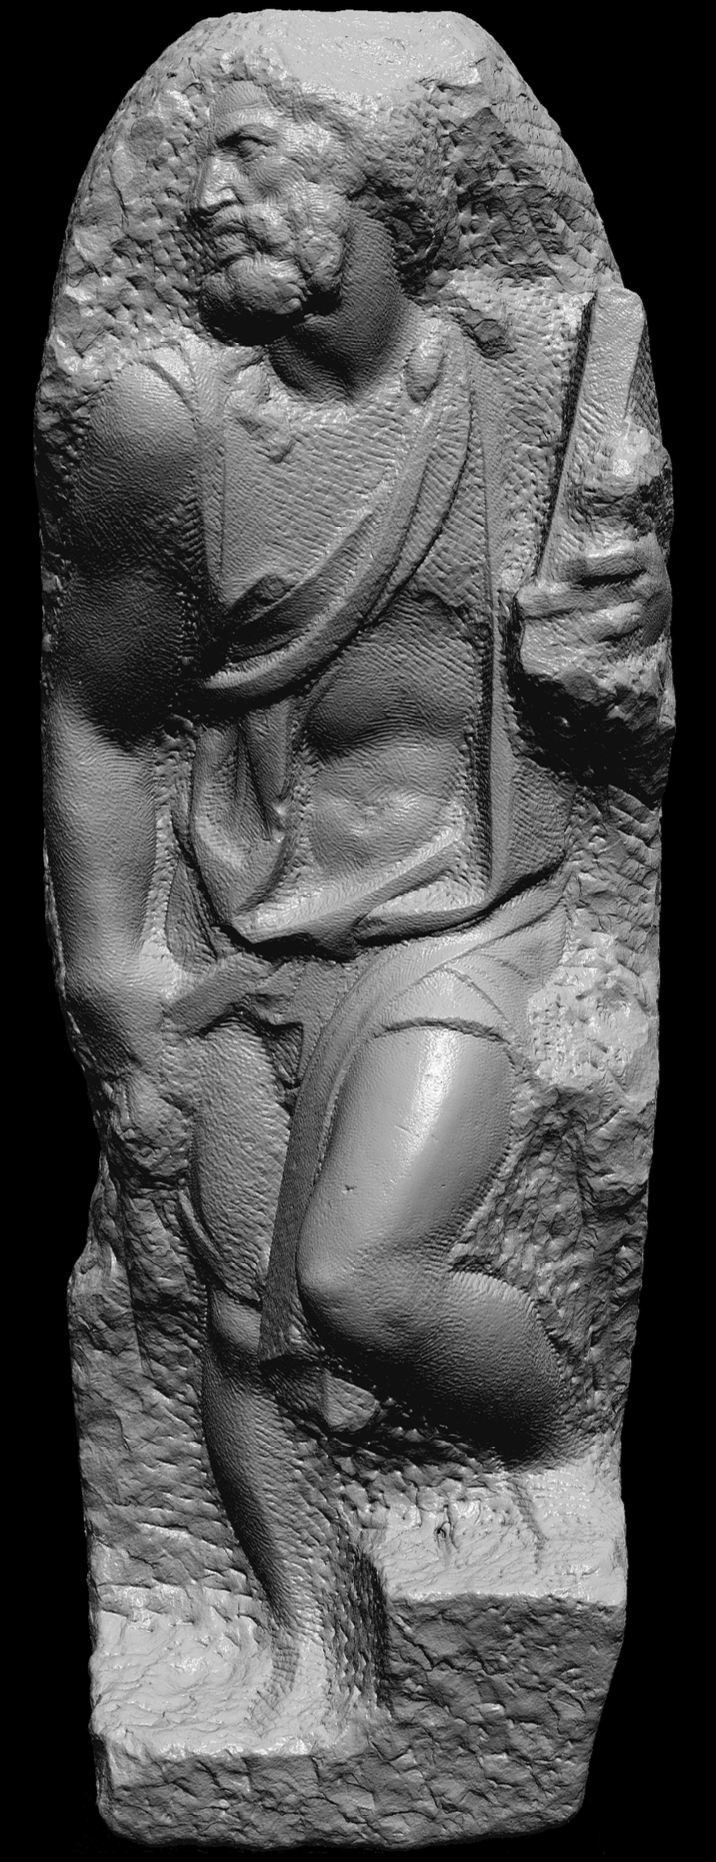
\includegraphics[height=9cm]{figures/chapter2/michelangelo_figure9.png}
\caption{Image 1: The Cyberware gantry standing next to Michelangelo's David / Image 2: Computer rendering of Michelangelo's St. Matthew showing preserved chisel marks at 0.29mm resolution. Source: \citet{levoy2000}}
\label{fig:michelangelo_gantry}
\end{figure}

The 2003 UNESCO Convention for the Safeguarding of Intangible Cultural Heritage marked a shift in this perspective by recognizing that cultural heritage extends beyond tangible things to include "identification, documentation, research, preservation, protection, promotion, enhancement, transmission" \citep{unesco2003}. More importantly, the convention defines intangible cultural heritage as something that is "constantly recreated by communities and groups in response to their environment" \citep{unesco2003}, explicitly acknowledging its living, evolving nature.

\vspace{0.5cm}

However, this framework still emphasizes documenting and officially recognizing traditional practices rather than preserving communities' ability to adapt and change those practices. The UNESCO approach, while acknowledging living practices, still requires processes that tend to crystallize traditions into documentable forms rather than preserving their adaptive capacity, the quality that democratic fabrication systems must maintain to enable ongoing maker authority over creative processes.

\subsection{Cross-Cultural Models of Adaptive Preservation}

The static documentation approaches critiqued highly contrast with preservation practices across different cultural contexts that prioritize maintaining agency and adaptive capacity over material authenticity. These alternative models demonstrate how preservation can support the kind of ongoing democratic authority that participatory fabrication requires.

\subsubsection{Cuban Automobile Preservation: Functionality Through Adaptation}

Cuba's preservation of classic American automobiles exemplifies a functional preservation, the maintainance of cultural significance through continuous adaptation oposed to static conservation. Following the 1959 Cuban Revolution and subsequent U.S. embargo, Cubans maintained an estimated 60,000 classic American cars through creative adaptation. As the \citet{diplomatictimes2019} reports, "About half of the cars originate from the 1950s, while 25 percent are from the 1940s and another 25 percent are from the 1930s. A lot of them have been passed down from generation to generation, along with the mechanical genius."

\begin{figure}[H]
\centering
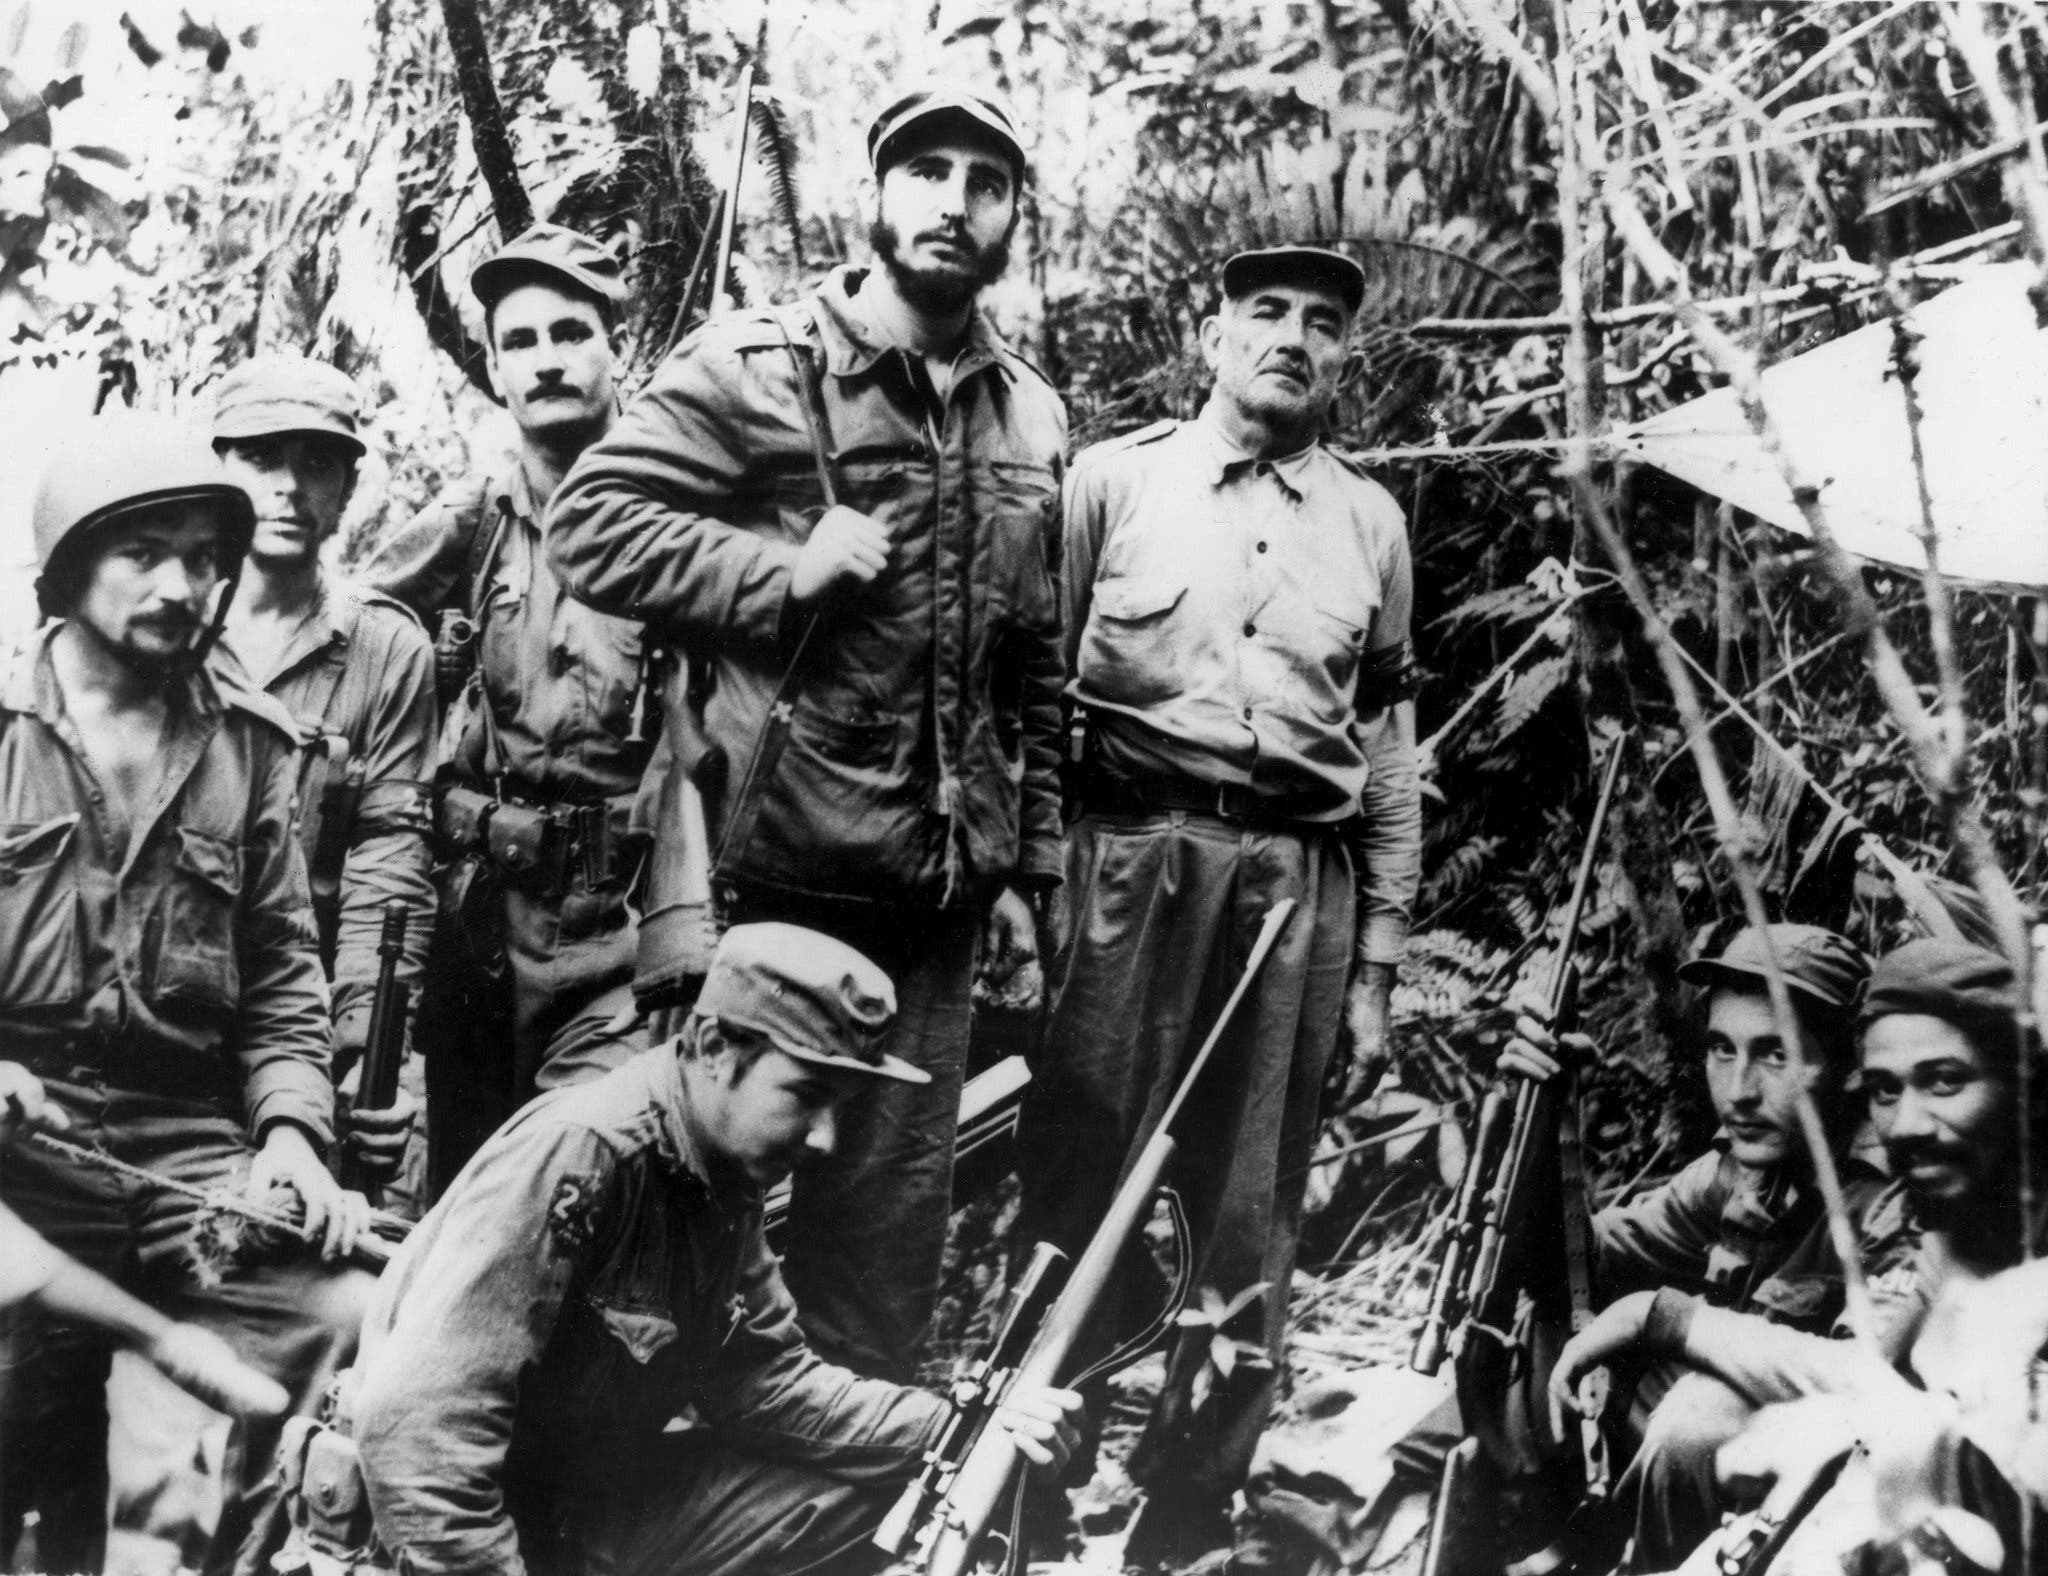
\includegraphics[height=5.6cm]{figures/chapter2/castro1.jpg}
\hspace{0.01cm}
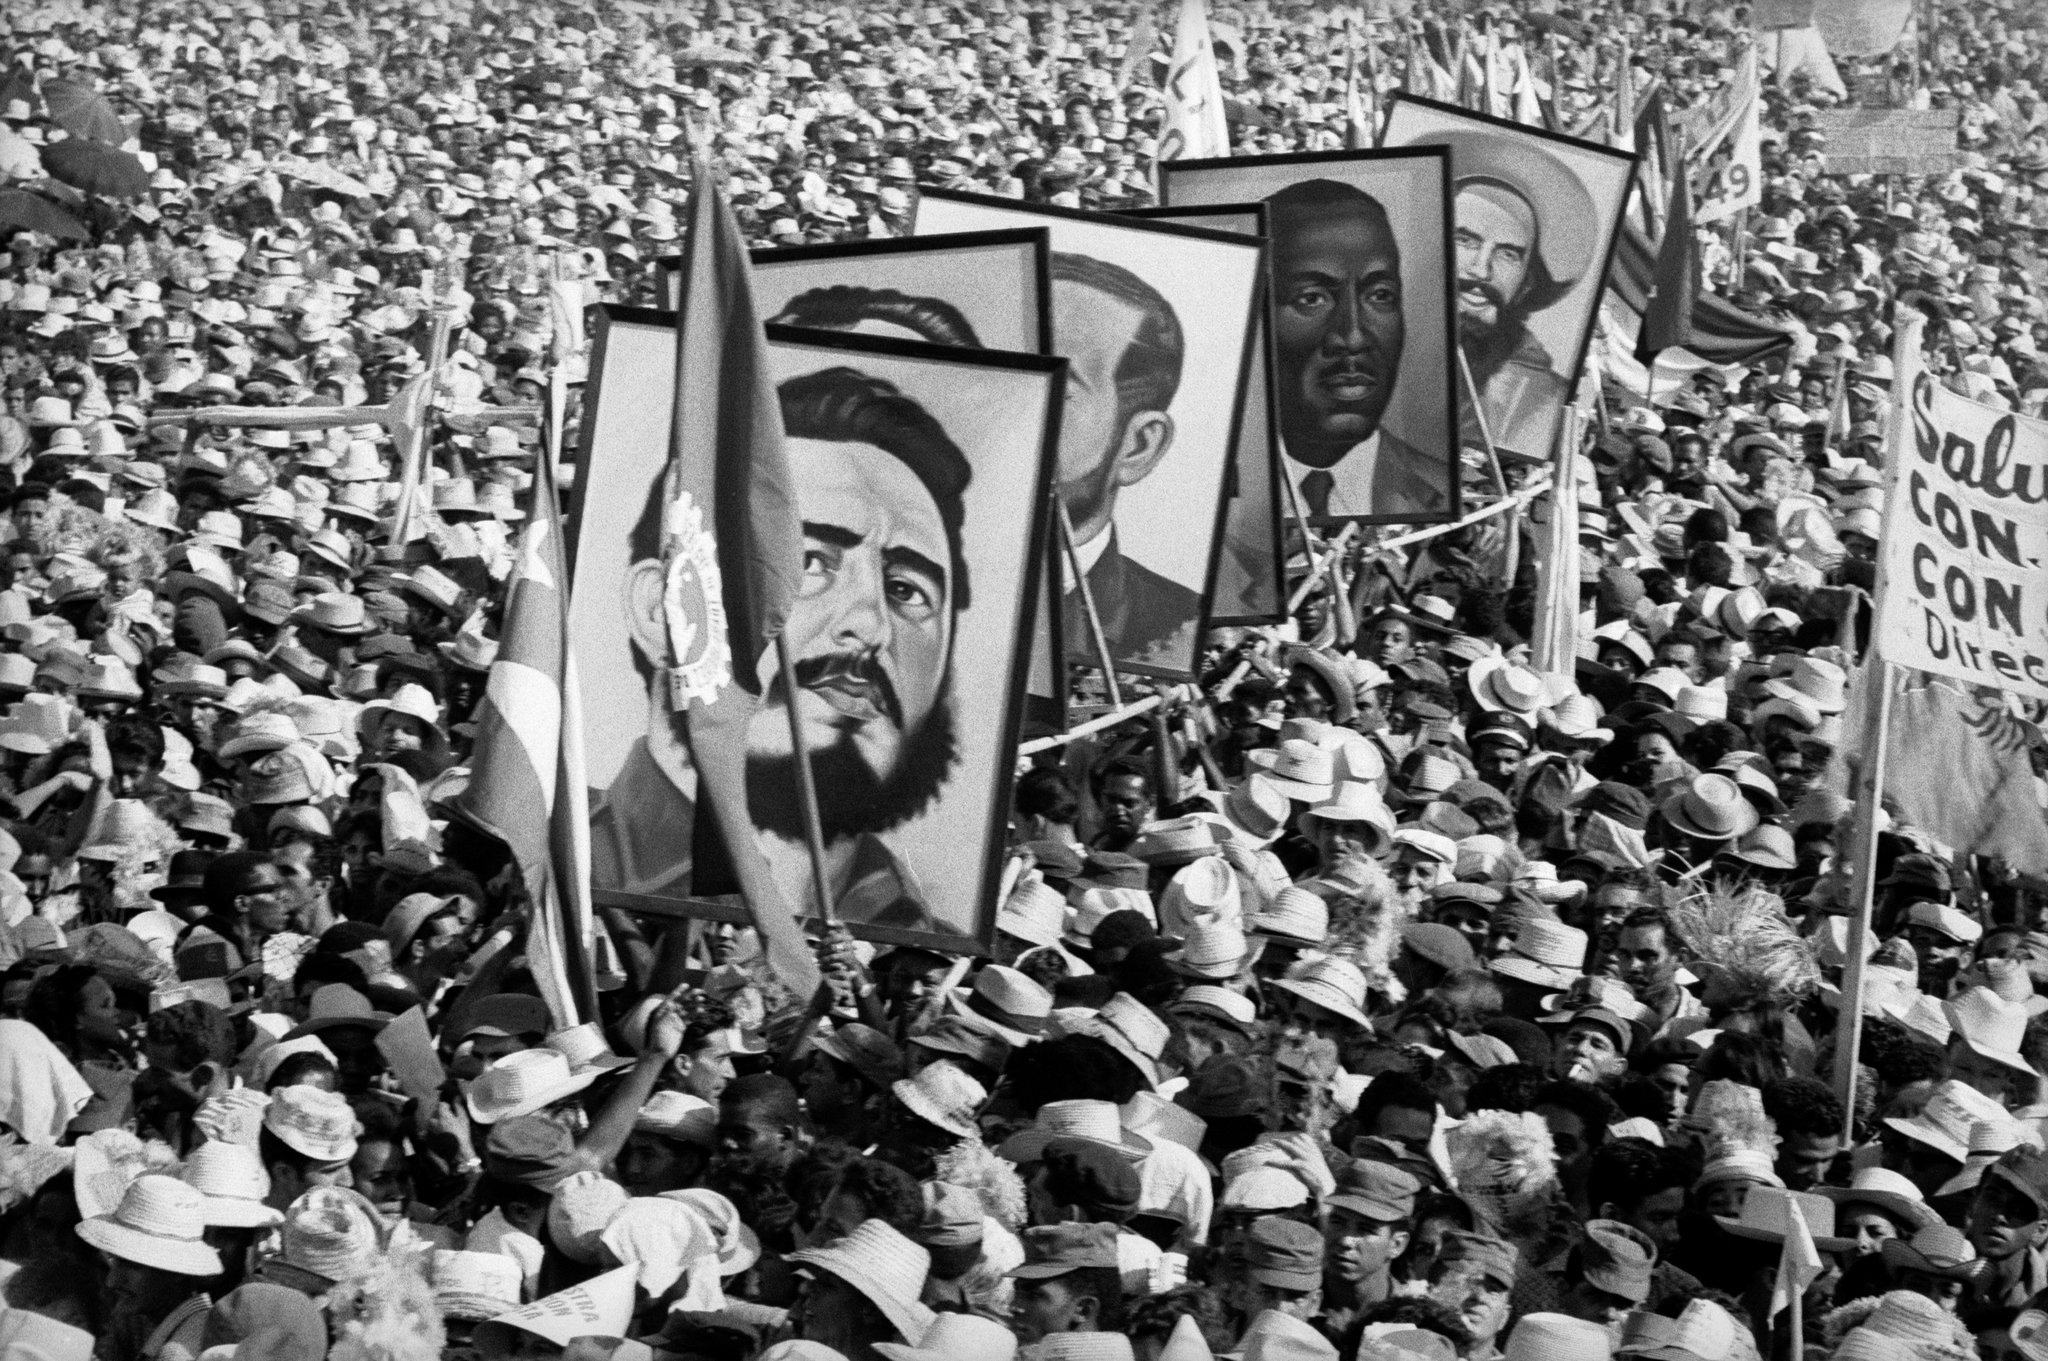
\includegraphics[height=5.6cm]{figures/chapter2/castro2.jpg}
\caption{Fidel Castro during the Cuban Revolution period, demonstrating the historical context that led to Cuba's unique preservation practices. Source: \citet{castro_time_photos}}
\label{fig:castro_revolution}
\end{figure}

These vehicles remain culturally significant not despite their modifications but because of them. Their external appearancespreserve historical recognition value while their internal systems have evolved into hybrid assemblages. "A common substitution on the old 1950s era cars on the island are diesel engines for the old straight-six or V-8 engines originally in the cars, due to diesel's lower cost on the island, and the better fuel efficiency of the engines," \citep{diplomatictimes2019} with "diesel engines from Russian trucks or boats" \citep{diplomatictimes2019} replacing original components.

\begin{figure}[H]
\centering
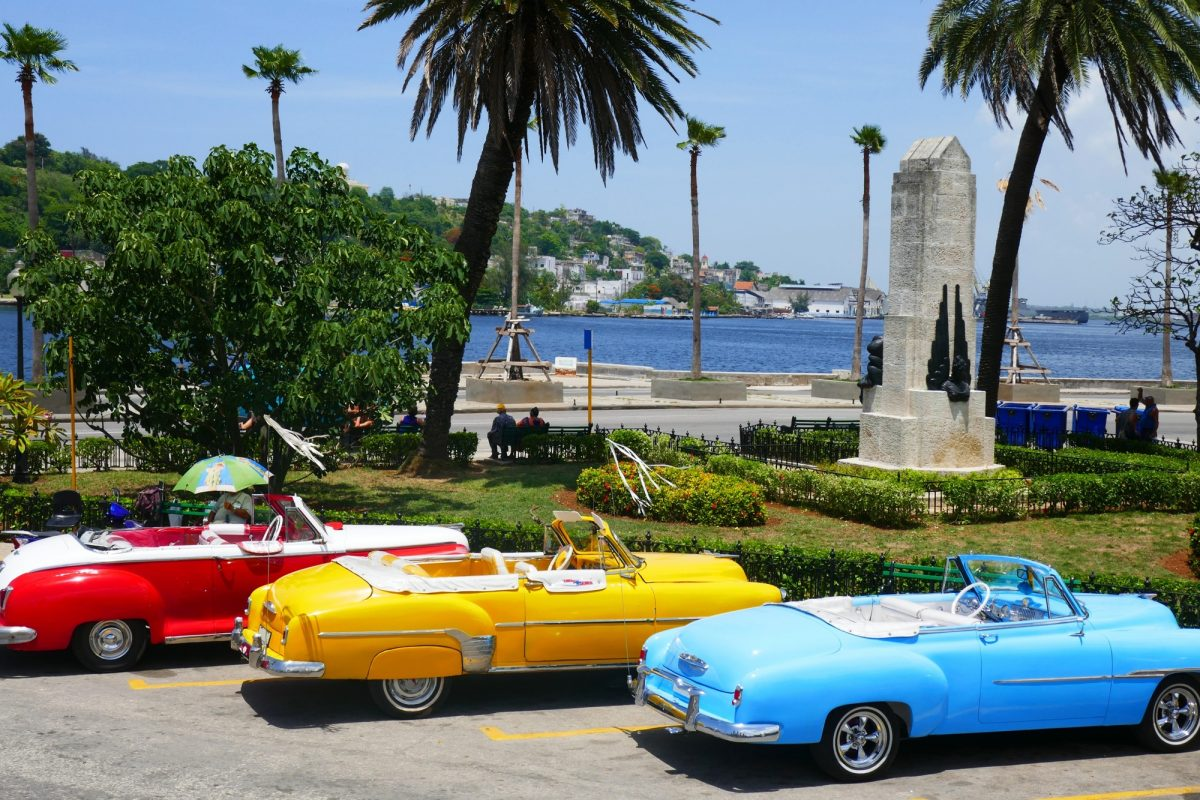
\includegraphics[width=1\textwidth]{figures/chapter2/vintage_autos_havana.jpeg}
\caption{Vintage 1950s American cars in Havana, Cuba, demonstrating functional preservation through continuous adaptation. Source: \citet{zerobyte2018}}
\label{fig:vintage_cars_havana}
\end{figure}

This preservation approach prioritizesthe ongoing functionality and cultural continuity over "strict" tangible authenticity. The cars remain integrated within contemporary Cuban life, functioning as taxis and tourist attractions rather than museum pieces, showcasing preservation through active use rather than protection from use. As \citet{adewale2024} observes, "While some people might expect these old cars to be museum pieces, they're part of everyday life in Cuba."

\subsubsection{Māori River Preservation: Relational Continuity Through Legal Innovation}

New Zealand's legal recognition of the Whanganui River as a living entity with "the same rights and responsibilities as a person" \citep{paremata2017} exemplifies preservation through transformed conceptual frameworks rather than material conservation. This approach emerged from Māori understanding expressed in the saying "Ko au te awa, ko te awa ko au" (I am the river, and the river is me), where the river name "Awa Tupua" includes "the whole river system, its spirit, and the people that are related to it" \citep{nationallibrarynz2017}.

\begin{figure}[H]
\centering

\includegraphics[width=1\textwidth]{figures/chapter2/whanganui.jpg}
\caption{River flowing through the Whanganui National Park. The Whanganui River was granted legal personhood in 2017, exemplifying relational preservation approaches that maintain living connections rather than static conservation. Source: \citet{paremata2017}}
\label{fig:whanganui_river}
\end{figure}

Rather than treating the river as a natural resource requiring protection through regulatory restriction, this model empowers the Māori to manage and protect the river based on their traditional ecological knowledge. As \citet{vijaykuma2019} notes, "As a consequence of this recognition, the Maori are now empowered to manage and protect the river based on their traditional ecological knowledge." Preservation here operates through maintaining relationships and ongoing interactions rather than controlling physical attributes or preventing change.

\vspace{0.5cm}

This relational approach recognizes that preservation must account for living connections between people, practices, and environments rather than treating cultural elements as discrete objects requiring isolation from contemporary influences.

\subsubsection{Implications for Digital Fabrication Democratization}

These diverse preservation models highlight shared principles that might address the democratization challenges identified earlier. Both Cuban functional adaptation and Māori relational continuity prioritize process over product, relationships over artifacts, and adaptation over stasis. As \citet{munoz_zanon_2025} concludes from this analysis, effective preservation approaches should "capture process knowledge and decision-making rather than just final geometries, preserve the dynamic relationship between maker, material, and tool, and allow for adaptation and evolution rather than freezing techniques in time."

\vspace{0.5cm}

Taking a look at the fabrication democratization aspect, out of these principles it can be asummed that preserving makers' agency requires organizational structures that maintain what the Cuban model showcases: the capacity for ongoing functional adaptation in response to changing conditions. Similarly to the Māori approach, genuine fabrication democratization would preserve makers' collective authority to determine how systems evolve, maintaining the relational continuity between human intention and material response.

\section{Documentation as Process Preservation}

The preservation approaches demonstrated by Cuban mechanics and Māori river stewardship raise questions about how digital fabrication systems might maintain makers' adaptive authority. These become particularly present when examining how fabrication knowledge is documented and transmitted. Current fabrication documentation perpetuates the technocratic representation characteristic of the distributed agency model, enabling participation within predetermined procedures while eliminating authority over how those procedures operate. Standard fabrication documentation (CAD files, parameter lists, step by step tutorials\dots) work as expert-designed interfaces that mediate between human intention and execution, eliminating opportunities for creative input beyond initial design specification.

\vspace{0.5cm}

However, examining documentation practices across different contexts reveal alternative approaches that align better with the dynamic preservation principles and participatory democratic theory already examined.

\subsection{Educational Documentation: Capturing Learning Processes}

The FabAcademy\footnote{FabAcademy is a global distributed educational program that teaches digital fabrication skills through hands-on learning and peer-to-peer collaboration. Students work through weekly assignments using local Fab Lab equipment while documenting their progress online.} and Fabricademy\footnote{Fabricademy is a transdisciplinary course that focuses on the development of new technologies and materials for the textile and fashion industry, emphasizing bio-fabrication, digital manufacturing, and sustainable design practices.} documentation sites provide examples of documentation that capture learning processes besides just technical outcomes. Unlike traditional technical manuals that present polished procedures, these educational platforms require students to document their entire learning journey, including failed experiments, debugging processes, and iterative refinements. Students document not only successful fabrication outcomes but also the problem-solving processes that led to those outcomes, creating records of adaptive authority.

\vspace{0.5cm}

Fabricademy specifically, becomes an interesting example as it extends this approach to textile and bio-material fabrication, where material unpredictability requires even greater adaptive capacity. Students document experiments with living materials and organic processes where following predetermined procedures often fails, and creative adaptation becomes essential. The resulting documentation captures the iterative process of material negotiation that can also be seen in traditional craft knowledge.

\subsection{Workflows as Narrative Preservation}

Tandem system \citep{tran_oleary_tandem_2024} represents another interesting approach to process-oriented documentation, implementing entire fabrication workflows as computational notebooks that preserve the complete narrative of creation. Rather than abstracting away the making process into separate CAD/CAM phases, Tandem maintains continuity between design decisions and material execution through "reproducible fabrication workflows" \citep{tran_oleary_tandem_2024}.

\vspace{0.5cm}

Interestingly, the project acknowledges that reproduction is not repetition, each implementation involves contextual adaptations based on available materials, equipment variations, and maker expertise. By implementing workflows as modifiable programs rather than fixed procedures, the system enables a generative reproduction, allowing to maintain creative agency while building on previous work, representing a significant switch from standard CAD/CAM workflows that concentrate creative decisions in separate design phases.

\section{The Limits of Algorithmic Preservation}

While these educational documentation approaches highlight promising alternatives to static preservation, they still operate within digital systems that fundamentally assume craft knowledge can be captured and transmitted through explicit documentation. This assumption has led contemporary approaches toward an even more technologically intensive solution: artificial intelligence and machine learning as comprehensive approaches to preserving and transmitting embodied knowledge. Suggesting that if human documentation proves inadequate, computational systems might decode the embodied knowledge through pattern recognition and data analysis.
\vspace{0.5cm}

However, machine learning approaches to kowledge preservation create a paradox: the more precisely algorithms attempt to measure and classify skilled practice, the more they help discover dimensions of that practice that resist an algorithmic categorization. This suggests that the problem with embodied knowledge preservation may not be inadequate computational architectures, but rather the conceptual framework that treats embodied knowledge as extractable data rather than contextual relationships between makers, materials, and tools.

\subsection{Testing the Limits of preservation. AI.RTISANSHIP}

Even with the aforementioned problems with algorithmic approaches to craft preservation, these "limitations" demanded empirical investigation. If computational systems truly cannot capture the adaptive authority that democratic making requires, this assumption needed testing through direct experimentation. To investigate these limitations empirically, this research developed as a first intervention the AI.RTISANSHIP experiment, an attempt to capture and digitize traditional pottery techniques through computer vision and machine learning systems, designed not to succeed but to reveal precisely where and why such approaches fail.

\vspace{0.5cm}

The goal was to create a machine learning model capable of analyzing artisanal hand movements and providing real-time feedback on the correctness of performed actions, essentially functioning as a "digital master" for craft learning. By pushing algorithmic preservation to its technical limits, the experiment aimed to identify the specific dimensions of craft knowledge that resist computational capture, thereby informing alternative future approaches.

\subsection{Technical Developement: Digitizing Embodied Knowledge}

The AI.RTISANSHIP system made use of MediaPipe's holistic model to track 33 pose landmarks, 21 landmarks per hand, and facial features, generating 225-dimensional vectors for each frame of movement. The machine learning pipeline processed sequences of 30 frames (approximately one second of movement) through a three layer bidirectional LSTM network with dropout regularization and L2 penalty terms to prevent overfitting.

\vspace{0.5cm}

Data collection involved recording multiple pottery throwing sessions, manually labeling frame collections of movements as "correct" or "incorrect," and training the neural network to recognize these patterns in unseen views. The system achieved accuracy in distinguishing between predefined movement categories, successfully identifying differences between throwing techniques and providing real-time classification through a web interface.

\vspace{0.5cm}

However, this technical "success" started highlighting conceptual issues mentioned before that only became apparent through the extended testing with the potters.

\subsection{The "Unmeasurable" Dimensions of Knowledge}

The experiment's concluded that craft knowledge works through dimensions that resist algorithmic capture. Computer vision could detect hand positions with great precision but remained blind to the tactile feedback that made those positions, the subtle resistance of clay indicating proper centering, texture changes indicating moisture, or vibrations warning of collapsation. These sensory channels, essential for pottery practice, exist entirely outside the visual domain that computer vision systems can access.

\vspace{0.5cm}

Beyond these sensory limitations, the experiment exposed deeper problems with the assumption that skilled practice follows standardizable patterns. Each participating artisan showcasded different approaches to identical pottery tasks, reflecting not just technical variations but personal relationships with clay developed through years of individual practice. Where one potter might relied on strong decisive movements, another employed gentle, patient techniques. These differences stemmed not from varying levels of skill but from unique personal histories, physical capabilities, and aesthetic preferences that had developed into distinct making "philosophies".

\vspace{0.5cm}

In it's core, the machine learning system's requirement for binary classification ("correct" versus "incorrect") proved conceptually inappropriate for pottery practice. The participating potters emphasized that successful throwing depends on continuous adaptation to emergent material conditions rather than adherence to predetermined techniques. This adaptive capacity, cannot be reduced to pattern recognition algorithms that require standardized input categories. Where pottery expertise emerges from continuous dialogue between maker and material, the AI system imposed predetermined classifications that eliminated precisely the adaptive responsiveness that characterizes skilled practice.

\subsection{Implications for Digital Fabrication Preservation}

The real-time feedback mechanism (color-coded overlays indicating "correct" or "incorrect" movements) created additional problems that highlighted even further the inadequacy of the approach. The potters, despite acknowledging the potential of the tool for educational purposes, reported that the visual feedback disrupted their attention to tactile cues. The system's focus on visual movement patterns diverted attention from the sensory channels through which pottery expertise actually operates.

\vspace{0.5cm}

The attempt to extract explicit rules from embodied practices assumes that skilled knowledge can be decomposed into discrete, transferable components. Yet the experiment, as was guessed before starting it, demonstrated that pottery expertise exists not in specific movements but in the capacity for contextual adaptation, precisely what the machine learning system eliminated through its standardized classifications.

\vspace{0.5cm}

Out of these findings, it is possible to suggest that effective craft preservation cannot operate through documentation technologies that abstract away material context and environmental variation.

\vspace{0.5cm}

Effective preservation, would need to maintain the conditions for adaptive response rather than understanding standardized procedures. Representing a shift from traditional documentation based approaches towards a preservation method that maintain the organizational structures only, enabeling ongoing creative adaptation.

\subsection{Beyond Documentation: Toward Ecological Preservation}

Experiment's limitations do not suggest fully abandoning documentation altogether, but rather reconceptualizing what documentation means within embodied knowledge preservation contexts. Documentation remains essential, but it must acknowledge that each implementation of documented knowledge will necessarily differ based on contextual variables, material conditions, and individual maker characteristics.

\vspace{0.5cm}

Rather than attempting to capture universal techniques through computational standardization, effective preservation requires documentation frameworks that explicitly account for contextual variation. This involves creating technological environments that preserve not just movement patterns but the decision-making processes that inform adaptive responses to changing conditions. Such systems would document the reasoning behind technical choices, the environmental factors that influence material behavior, and the range of acceptable variations rather than singular "correct" procedures.

\vspace{0.5cm}

This contextual approach to documentation would treat preservation as the maintenance of conditions for ongoing creative adaptation. Digital fabrication systems (or workflows) designed according to these principles would preserve material feedback channels, enabling real-time modification based on emergent conditions, and maintain maker authority. Documentation would function as a scaffold for contextual learning rather than a template for mechanical reproduction.

\vspace{0.5cm}

The following chapters will explore how such contextually-aware preservation might operate within digital fabrication workflows, building on the AI.RTISANSHIP experiment's insights to develop newer approaches for preservation, reflecting the unique intersection of maker, material, and circumstance.































































